% Name: SR latch
% Description: Two cross-coupled NOR gates that hold one bit, with set and reset inputs and the outputs Q and Q̄, beside the latch's truth table.
% Tags: SR latch, NOR gate, flip-flop, memory, sequential logic

\usetikzlibrary{circuits.logic.US}

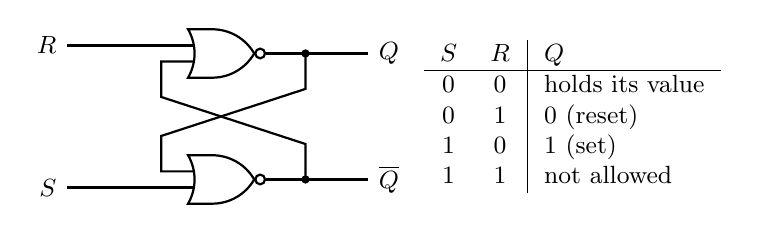
\begin{tikzpicture}[circuit logic US, thick, every circuit symbol/.style={thick}, every node/.style={font=\small}]
  \node[nor gate] (n1) at (2.5,1.6) {};
  \node[nor gate] (n2) at (2.5,0) {};
  \draw (n1.input 1) -- ++(-1.6,0) node[left] {$R$};
  \draw (n2.input 2) -- ++(-1.6,0) node[left] {$S$};
  \draw (n1.output) -- ++(1.3,0) node[right] {$Q$};
  \draw (n2.output) -- ++(1.3,0) node[right] {$\overline{Q}$};
  % Each output feeds back to the other gate's free input; the two wires cross without joining
  \draw (n1.output) ++(0.5,0) coordinate (q) -- ++(0,-0.45) -- ($(n2.input 1) + (-0.4,0.45)$) |- (n2.input 1);
  \draw (n2.output) ++(0.5,0) coordinate (qb) -- ++(0,0.45) -- ($(n1.input 2) + (-0.4,-0.45)$) |- (n1.input 2);
  \fill (q) circle (1.5pt) (qb) circle (1.5pt);
  \node[anchor=west] at (5,0.8) {%
    \begin{tabular}{cc|l}
      $S$ & $R$ & $Q$ \\ \hline
      0 & 0 & holds its value \\
      0 & 1 & 0 (reset) \\
      1 & 0 & 1 (set) \\
      1 & 1 & not allowed
    \end{tabular}};
\end{tikzpicture}
